\section{Models}
\label{sec:usedModels}

In this section all models are discussed which are used or created in this work.
This section is divided into three subsections.
Each of them corresponds to one of the main contributions of this work.
Therefore the first section gives a brief overview of used object detection models, the second one with the \ac{TEP}-Net \cite{tepNet2024} because it is used as a baseline.
Additionally, further improvements of this model are described in this section.
The last section describes all temporal models.

\subsection{Object Detection Models}

The state of the art in \autoref{sec:ObjectDetection} shows that one-stage detectors have the most promising characteristics to be successfully utilized in this work.
The most interesting ones are the models from the \ac{YOLO} series, especially the most recent ones because they focus on improved parameter usage.
This makes the models light weight and presents an advantage for this work, because operation on limited hardware is aimed for.
At the start of this work the most recent model from the \ac{YOLO} series is the \ac{YOLO}v9 \cite{YOLOv9}.
For object detection different models of the \ac{YOLO}v9 and the \ac{GELAN} series are available.
However, the \ac{YOLO}v9 models were not fully supported at that time.
Therefore the models used for experiments include the \ac{GELAN}-c and \ac{GELAN}-e.
These are obtained trough the GitHub repository \cite{YOLOv9GitHub} and used unchanged.
An additional model which is used for experiments is the \ac{YOLO}v7 \cite{yolov7} model, which is also utilized unchanged from the GitHub repository \cite{YOLOv7GitHub}.

\subsection{TEP-Net Model}
\label{subsec:baselineModel}

In the literature rails are often detected without distinction between all rails visible in an image and the rail the train continues.
\cite{tepNet2024} therefore proposes a regression-based approach, which restricts the model to predict a single track.
The idea comes from various lane detection methods in autonomous driving applications for road cars and is fitted to the rail domain.
Since, this method fits well to the goal of this work, it is used as a baseline for further experiments.

Although rails can be represented by second or third-degree polynomials most of the time \cite{PolyLaneNetRoad2021}, they may also take more complex geometric shapes.
Hence, limiting the output to presumed forms is discouraged.
Therefore, the method used in \cite{tepNet2024} employs spline interpolation to describe such complex structures.

\begin{figure}[H]
    \centering
    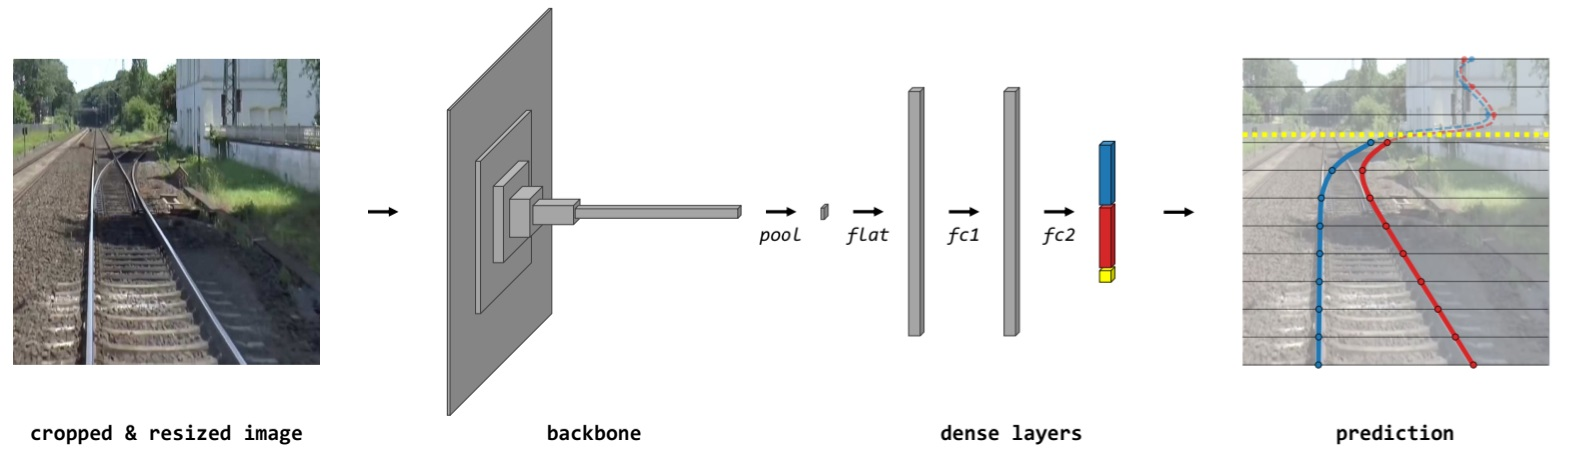
\includegraphics[width=\linewidth]{PICs/Baselinepaper/TEP-Net_model.jpg}
    \caption{\ac{TEP}-Net model architecture\cite{tepNet2024}. The input of the model is a cropped and resized image and the output of the model are the $x$-values for the left and right rail on each anchor line plus an additional value for the $y$-limit.}
    \label{fig:TEP-Net_model}
\end{figure}

As shown in the prediction of \autoref{fig:TEP-Net_model}, a set of horizontal lines are overlayed in the cropped image.
The number of $y$-lines or "anchors" is determined by a hyperparameter.
They are uniformly distributed along the $y$-axis. For each line, two $x$-values are predicted.
One for the left rail and one for the right rail.
The prediction image of \autoref{fig:TEP-Net_model} and the second and fourth images in the bottom row of \autoref{fig:tepNet_dataaugmentation} show that rails do not necessarily cross with anchor lines at the top of image crops.
Therefore, an additional $y$-limit is predicted, which gives information up to which anchor the rail should be detected.
Anchors and their $x$-values above this horizon line do not hold valuable information and are ignored.

For this novel regression task, a new model architecture is created.
For this model widely used backbone architectures like ResNet and EfficientNet are chosen.
The input of the backbones is an image crop with the size of $3 \times 512 \times 512$ which represents a rough average of crops obtained by data augmentation strategies.
These backbones extract relevant features from these crops reducing the spatial dimensions and increasing channel size to a high number.
After that, the feature map's number of channels is reduced to a predefined size with a 1x1 Conv2d layer \cite{pytorch_conv2d_docu} and flattened to a vector.
This feature vector serves as the input for the prediction head, which consists of two fully connected layers \cite{pytorch_linearLayer_docu} in series.
The size of the linear layers is set with a hyperparameter.
In the last layer, a reduction leads to the resulting prediction vector with the dimension $2 \times H + 1$.
This vector includes the entire information of one prediction.
$H$ is the number of anchors.
The first set of values with size $H$ is for the left rail, another $H$ set for the right rail and the $+ 1$ is for the last values being the horizon line.

This architecture's policy for value ranges does not restrict the $x$-values in any way.
This way predictions can be outside of a crop and the model can learn that sometimes the rails extend out of the viewed field.
The $y$-limit on the other hand is constrained to a range between 0 and 1 with a Sigmoid function.

The introduced model architecture can be classified as an end-to-end framework.
This means the model can be trained and used for inference without any steps in between.
It takes in raw data and results in a complete prediction.


\subsection{Improvements to the TEP-Net Model}
\label{subsec:improvemensts2BaselineModel}

One of the main contributions of this work is to improve the chosen baseline model from \cite{tepNet2024}.
These improvements can be roughly divided into three parts.
First, the backbones are exchanged with other architectures.
Secondly, after the backbones, a true pooling layer is integrated.
Thirdly, experiments with different prediction heads are conducted.
The following sections describe the structure of these architecture changes in detail.

\subsubsection{Backbones}
\label{subsubsec:backbones}

Backbones are used to extract features from images.
These are parts of \ac{CNN}s that input and output tensors.
Common \ac{CNN} architectures usually work with 4D tensors with $B \times C \times H \times W$ as shown in \autoref{fig:backboneLogic}.
$B$ is the batch size, $C$ is the channel size, $H$ and $W$ are the height and width of the input image.
The backbone transforms this high-level feature map into a low-level one with different operations, resulting in a tensor with a high number of channels $C$ and low numbers in resolution $H$ and $W$.
The batch size $B$ tells how many images the \ac{CNN} processes simultaneously and stays the same.
These characteristics apply to all four chosen backbones.
As described in the state of the art in \autoref{sec:networkArchitectures}, the most interesting models are ResNet \cite{ResNet}, EfficientNet \cite{EfficientNet}, DenseNet \cite{DenseNets}, and MobileNetV3 \cite{MobileNetV3}.
ResNet and EfficientNet are already implemented in \cite{tepNet2024}.
DenseNet and MobileNet are additionally integrated in this work.
\autoref{tab:backboneVersions} gives an overview of all different versions which are implemented in this work.

\begin{table}[H]
    \centering
    \begin{tabular}{|l|l|}
    %\begin{tabular}{| p{0.3\linewidth} | p{0.6\linewidth} |}
        \hline
        ResNet & 18, 34, 50\\
        \hline
        MobileNetV3 & small, large\\
        \hline
        DenseNet & 121, 161, 169, 201\\
        \hline
        EfficientNet & B0, B1, B2, B3\\
        \hline
    \end{tabular}
    \caption{Versions of backbones utilized in this work}
    \label{tab:backboneVersions}
\end{table}

\begin{figure}[H]
    \centering
    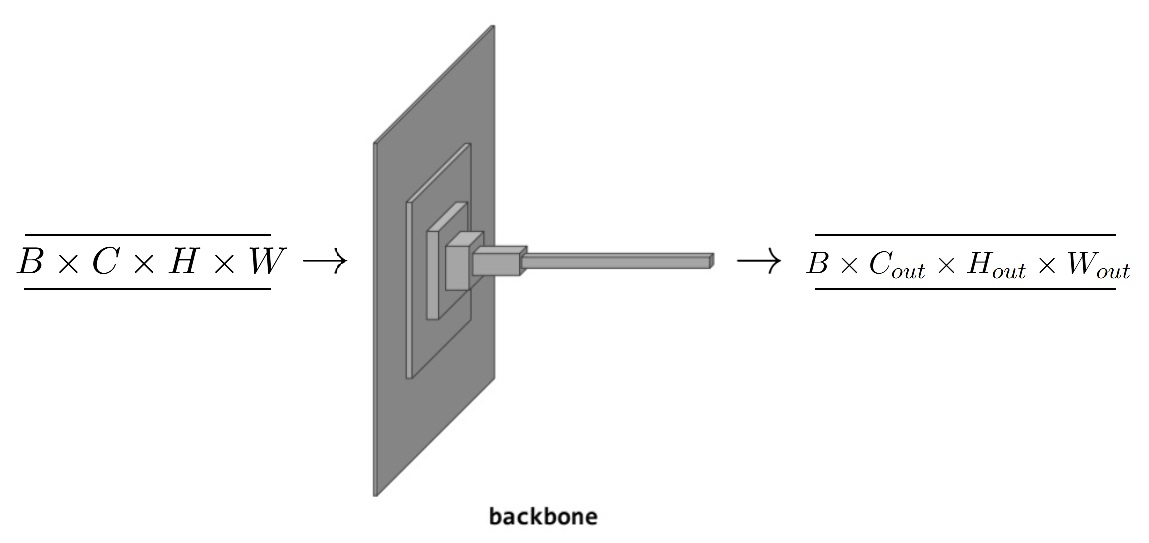
\includegraphics[width=0.6\linewidth]{PICs/improvedModel/backbone_logic.jpg}
    \caption{Backbone logic (Backbone graphic taken from \cite{tepNet2024}).}
    \label{fig:backboneLogic}
\end{figure}

When exchanging backbone architectures it is important, that the dimensions of input and output tensors are the same for every backbone otherwise the next layers would get different input dimensions than they are designed for.
Standardizing the input tensor is done by resizing an image to $512 \times 512$ after augmentation.
While $B$ is set by a hyperparameter, $C = 3$ because images are in the 3-channel \ac{RGB} format.
For the output dimensions, the backbone architectures and their operations must be analyzed.
When inspecting all four backbones in more detail it becomes clear that they all share the following characteristics:

\begin{itemize}
    \item The input resolution in all papers is $224 \times 224$.
    \item At the end, there is either a pooling layer, a $1 \times 1$ convolutional layer, or both in combination with fully connected layers forming a prediction head for classification tasks.
    \item Before the prediction head, the spatial resolution of feature maps is $7 \times 7$.
\end{itemize}

With this information, the last layers of each backbone can be discarded, so all backbones output tensors with the same $H$ and $W$.
In all four papers, the architecture transforms tensors with a resolution of $224 \times 224$ to a tensor with $7 \times 7$ before the prediction heads.
This means they all have the same reduction factor of 32.
Since the input resolution of $512 \times 512$ is used in this work resulting feature maps have a resolution of $16 \times 16$ after backbones.
The exact dimensions of all tensors are shown in \autoref{tab:backboneDimensions}.

\begin{table}[H]
\centering
\begin{tabular}{|r|p{0.2\linewidth}|r@{ }r@{,  }r@{,  }r@{,  }r@{ }l|}\hline
%\begin{tabular}{| p{0.3\linewidth} | p{0.3\linewidth} | p{0.3\linewidth} |}\hline
\multicolumn{1}{|l|}{\textbf{Backbone}}       & \textbf{Input dimensions} & \multicolumn{6}{|l|}{\textbf{Output dimensions}}\\\hline
ResNet                  & \multirow{4}{=}{\centering [ 8, 3, 512, 512 ]}  & [ & 8 &  512 & 16 & 16 &]\\\cline{1-1} \cline{3-8}
MobileNetV3             &                                               & [ & 8 &   96 & 16 & 16 &]\\\cline{1-1} \cline{3-8}
DenseNet                &                                               & [ & 8 & 1024 & 16 & 16 &]\\\cline{1-1} \cline{3-8}
EfficientNet            &                                               & [ & 8 &  384 & 16 & 16 &]\\\hline
\end{tabular}
\caption{Input and output dimensions of backbones utilized in this work}
\label{tab:backboneDimensions}
\end{table}

\subsubsection{Pooling Layer}

In \autoref{subsubsec:backbones} the spatial resolution is standardized across multiple backbones.
However, \autoref{tab:backboneDimensions} shows that after different backbones different numbers of channels $C$ are obtained.
To solve this and make the backbones interchangeable, \cite{tepNet2024} proposed a pooling layer at the start of the prediction head.
However, when analyzing the code \cite{tepNet2024GitHub}, it becomes clear that \cite{tepNet2024} used a convolution with a $1 \times 1$ kernel instead of a pooling.
This \textit{conv2D1x1} transforms the feature map of the backbone to a predefined channel size.
In \cite{tepNet2024GitHub} it is set to 8, resulting in the dimensions $8 \times 16 \times 16$.
Then this feature map is flattened to a vector for further processing with fully connected layers.

A critical positional encoding is missed when directly flattening this feature map.
Therefore in this work after standardizing the dimensions with the \textit{conv2D1x1} layer, a true pooling layer is integrated.
This additional layer consists of either an adaptive average pooling \cite{pytorch_averagePool_docu} or an adaptive max pooling \cite{pytorch_maxPool_docu}.
An additional encoding takes place resulting in a vector-like tensor with dimensions $C \times 1 \times 1$.
Besides the extra positional encoding, a further gained advantage is that the structure of data stays the same when flattening this feature map to a vector.

\begin{figure}[H]
    \centering
    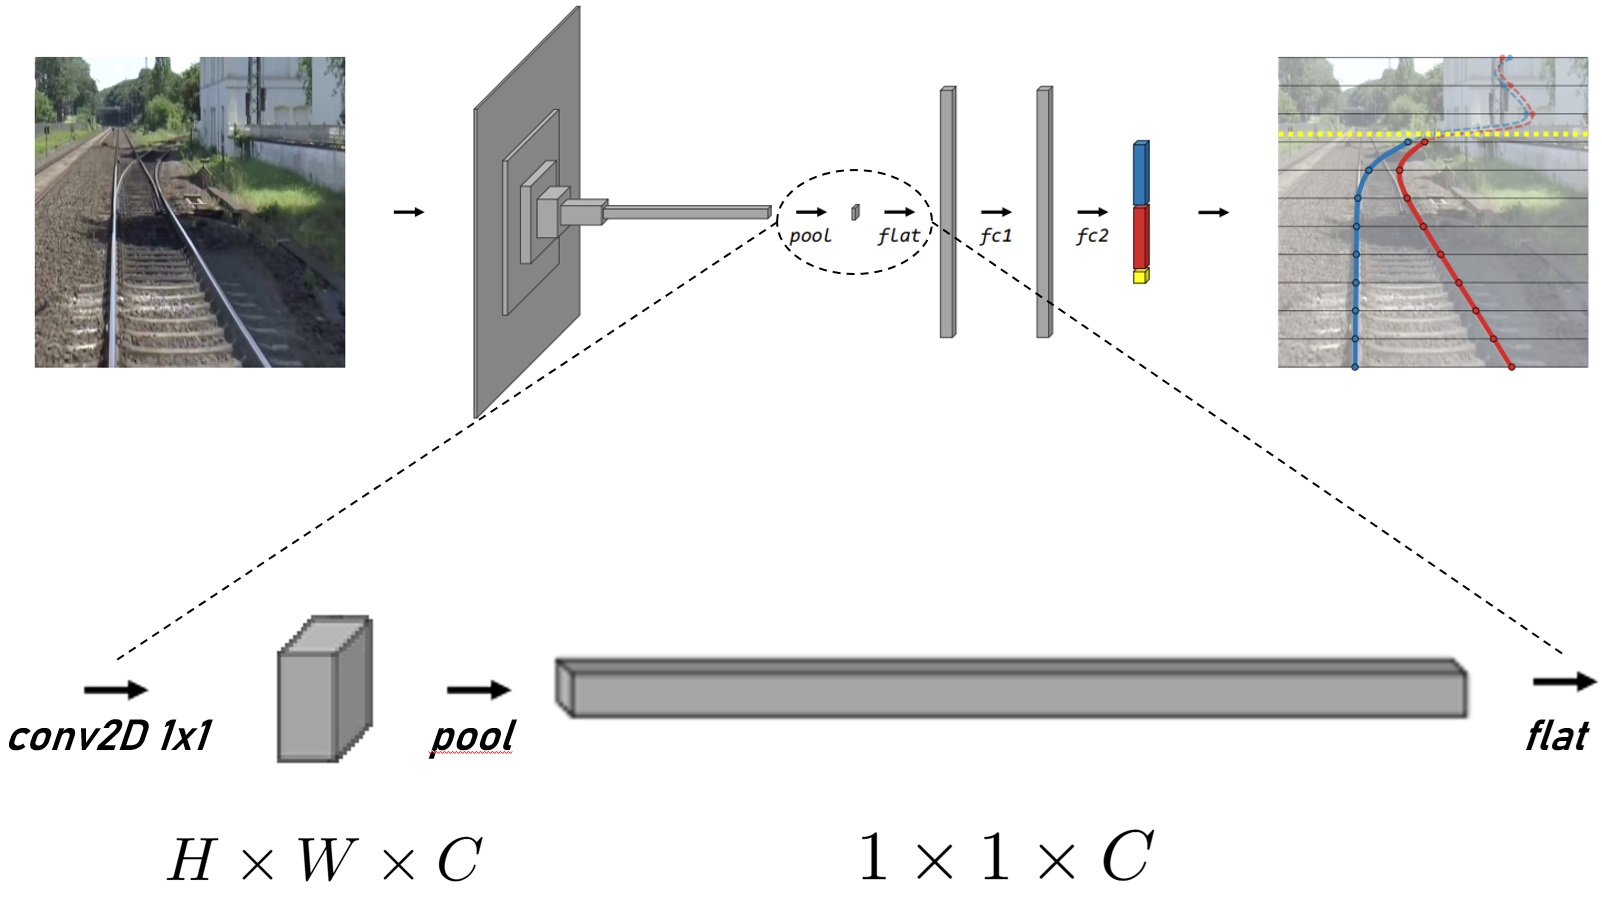
\includegraphics[width=0.75\linewidth]{PICs/improvedModel/poolingLayers.jpg}
    \caption{Integration of a true Pooling Layer (Model graphic taken from \cite{tepNet2024} and changed).}
    \label{fig:truePoolingLayer}
\end{figure}

\subsubsection{prediction Heads}

Another improvement to \ac{TEP}-Net \cite{tepNet2024} is a different prediction head.
Experiments are conducted with four variations of architectures shown in \autoref{fig:differentpredHeads}.

\begin{figure}[H]
    \centering
    \begin{subfigure}[t]{0.21\textwidth}
        \centering
        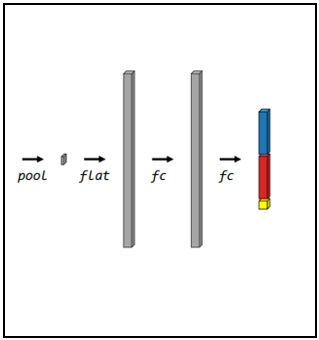
\includegraphics[height=3.3cm, keepaspectratio]{PICs/improvedModel/originalHead.jpg}
        \caption{Original Head \cite{tepNet2024}}
        \label{fig:predHeadOriginal}
    \end{subfigure}
    \begin{subfigure}[t]{0.27\textwidth}
        \centering
        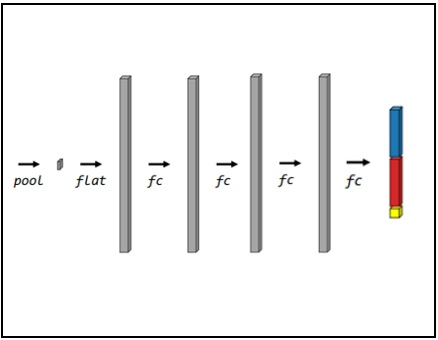
\includegraphics[height=3.3cm, keepaspectratio]{PICs/improvedModel/depthHead.jpg}
        \caption{Depth Head}
        \label{fig:predHeadDepth}
    \end{subfigure}
    \begin{subfigure}[t]{0.24\textwidth}
        \centering
        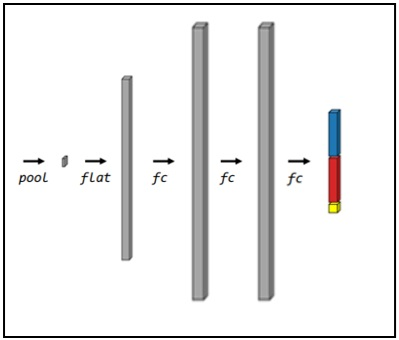
\includegraphics[height=3.3cm, keepaspectratio]{PICs/improvedModel/widthHead.jpg}
        \caption{Width Head}
        \label{fig:predHeadWidth}
    \end{subfigure}
    \begin{subfigure}[t]{0.26\textwidth}
        \centering
        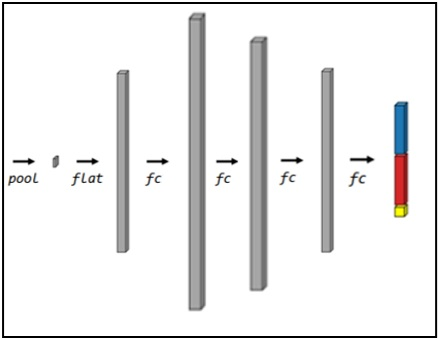
\includegraphics[height=3.3cm, keepaspectratio]{PICs/improvedModel/trapezHead.jpg}
        \caption{Trapeze Head}
        \label{fig:predHeadTrapez}
    \end{subfigure}
    \caption{Different architectures for prediction heads.}
    \label{fig:differentpredHeads}
\end{figure}

For comparison, the original head is displayed in \autoref{fig:predHeadOriginal}, which has 2 \ac{FC} layers \cite{pytorch_linearLayer_docu}.
The first one has input and output sizes of 2048 and the second one reduces the 2048 features to the output size $2 \times H + 1$ as explained in \autoref{subsec:baselineModel}.
The Depth and Width head, shown in \autoref{fig:predHeadDepth} and \autoref{fig:predHeadWidth} are inspired by the EfficientNet \cite{EfficientNet} scaling technique.
The Depth head increases the number of \ac{FC} layers to 4 and keeps the feature size at 2048.
The Width head doubles the feature size of layers.
Before that, a \ac{FC} layer gets the flattened feature vector from the backbone of site 2048 and increases it to 4096.
Then two wider \ac{FC} layers are used, while the second one reduces the features to the output size.
\autoref{fig:predHeadTrapez} shows the Trapeze head.
This had is named after its rough form and is a combination of the Depth and Width head.
First, it increases the number of features then it gradually compresses data until the last \ac{FC} layer reduces the size to the defined output.
The exact input and output size of each layer is shown in \autoref{tab:trapezHeadStructure}.
All heads use linear layers \cite{pytorch_linearLayer_docu} and \ac{ReLU} activation functions \cite{pytorch_relu_docu} in between visualized in \autoref{fig:ReLU}.

\begin{table}[H]
    \centering
    \begin{tabular}{|l|l|l|}
    %\begin{tabular}{| p{0.3\linewidth} | p{0.6\linewidth} |}
        \hline
        \textbf{Layers} & \textbf{Input size} & \textbf{Output size}\\
        \hline
        1. FC-Layer & 2048 & 3584 ($2048 \times 1.75$)\\
        \hline
        2. FC-Layer & 3584 & 2560 ($2048 \times 1.25$)\\
        \hline
        3. FC-Layer & 2560 & 2048\\
        \hline
        4. FC-Layer & 2048 & \(2 \times H + 1\)\\
        \hline
    \end{tabular}
    \caption{Detailed network structure of Trapeze Head}
    \label{tab:trapezHeadStructure}
\end{table}

\begin{figure}[H]
    \centering
    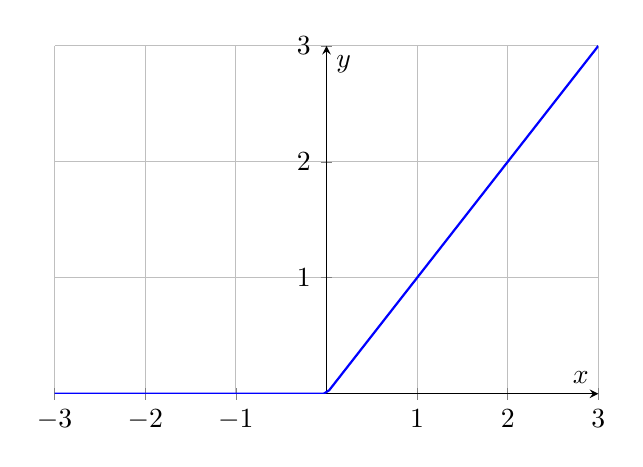
\begin{tikzpicture}
        \begin{axis}[
            axis lines=middle,
            xlabel={$x$},
            ylabel={$y$},
            domain=-3:3,
            samples=100,
            ymin=0, ymax=3,
            grid=both,
            %enlargelimits=true % zeigt nur jede 2 zahl an auf einer achse
            %xmin=-3, xmax=3, % Zoom Bereich auf der x-Achse
            width=0.7\textwidth, % Breitere Grafik
            height=6cm, % Schmalere Höhe der Grafik
        ]
            \addplot[blue, thick] {max(0, x)};
        \end{axis}
        \end{tikzpicture}
    \caption{$ReLU$ Activation Function \cite{pytorch_relu_docu}}
    \label{fig:ReLU}
\end{figure}

\subsection{Temporal Models}
\label{sec:temporalModels}

As described in \autoref{sec:limitationBaseline} there is a limitation to this model presented by the single-frame-based approach.
This becomes a disadvantage especially when focusing on switches.
While there are many possible approaches to dampen this issue, the most promising solution incorporates an \ac{RNN} in the model.
The \ac{RNN} module should consider the temporal component and learn the dependencies between successive frames.
Therefore, this \ac{CNN}-\ac{RNN} architecture inputs a video stream or in simpler terms, several consecutive frames instead of a single one.
Since the wanted prediction output is the same as the single-frame-based model, it stays the same.
This effectively makes this approach a sequence-to-one problem, in which only the output of the last frame is considered.
A schematic visualization is shown in \autoref{fig:schematicTemporalModel} in which the \ac{RNN} module is in the prediction head before the \ac{FC} layers.

\begin{figure}[H]
    \centering
    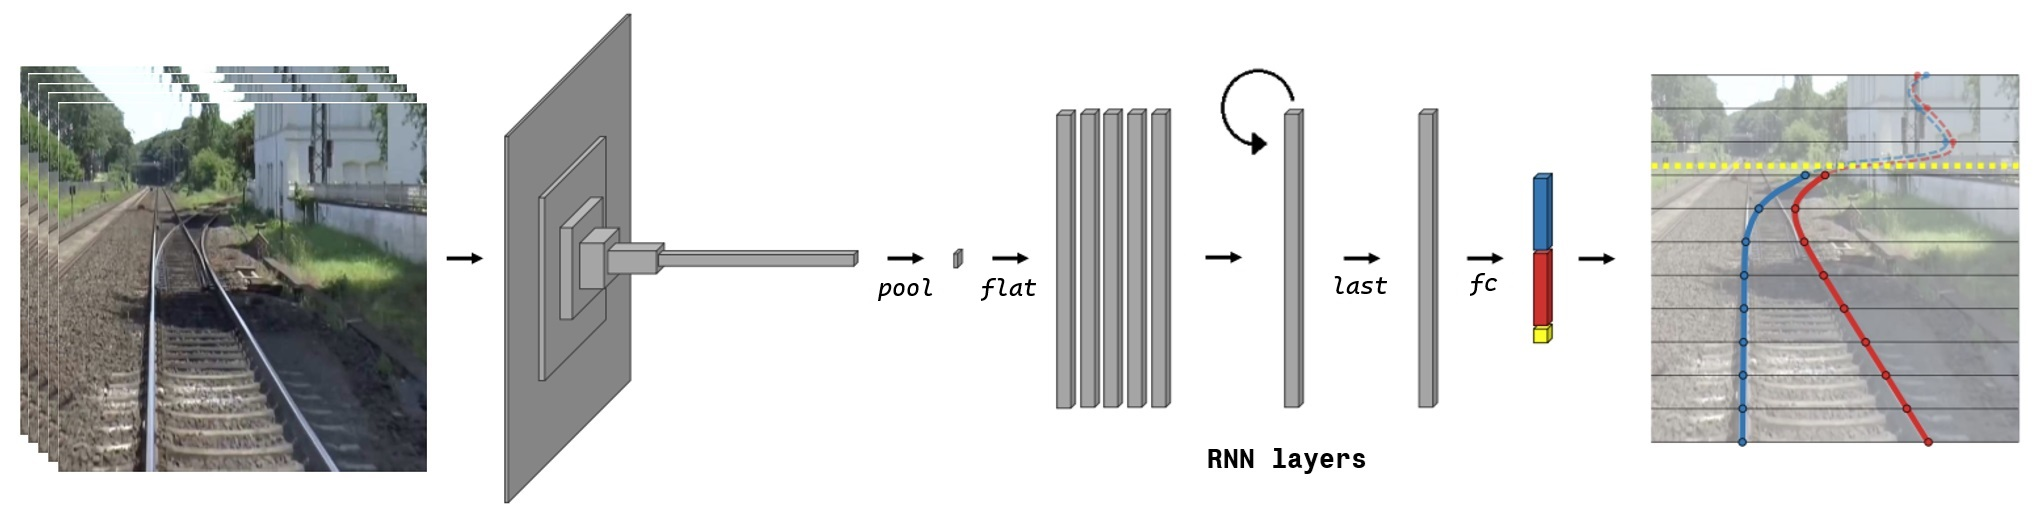
\includegraphics[width=\linewidth]{PICs//temporalModels/schematicDrawing.jpg}
    \caption{Schematic drawing of a temporal model with an integrated \ac{RNN} module (Graphic taken from \cite{tepNet2024} and changed).}
    \label{fig:schematicTemporalModel}
\end{figure}

The new problem formulation demands the development of new implementations and solutions.
However, the single-frame-based model shows satisfactory performance in almost every scenario except the ones including switches.
This led to the concept of reusing all parts of the single-frame-based model training, as long as the new temporal problem formulation allows for their re-usability.
Since the new formulation deals with a sequence-to-one problem, the output is on a single frame. This allows the loss function to be used as it is.
Another idea is to not waste any past experiments or model trainings.
Therefore, all temporal models use as many pre-trained weights as possible resulting in transfer learning approaches up to the point where in the model the temporal component is learned.
This means the weights from the best single-frame-based model are used for initialization.
Furthermore, in all experiments, backbones are frozen.
This strategy does not allow weights to be changed during training.
The idea is, that backbones are already trained to extract the most relevant features of images from single-frame-based trainings.

Following these rules leads to 8 different model structures, which have been trained and evaluated on a new dataset tailored for this use case.
There are two kinds of temporal models tested for this application.
The first kind incorporates \ac{RNN} modules.
For the second kind, the idea is to learn temporal dependencies only with \ac{FC} layers.
All models are visualized in \autoref{fig:temporalModels}.

\begin{figure}[H]
    \centering
    % Erste Zeile
    \begin{subfigure}[b]{0.48\textwidth}
        \centering
        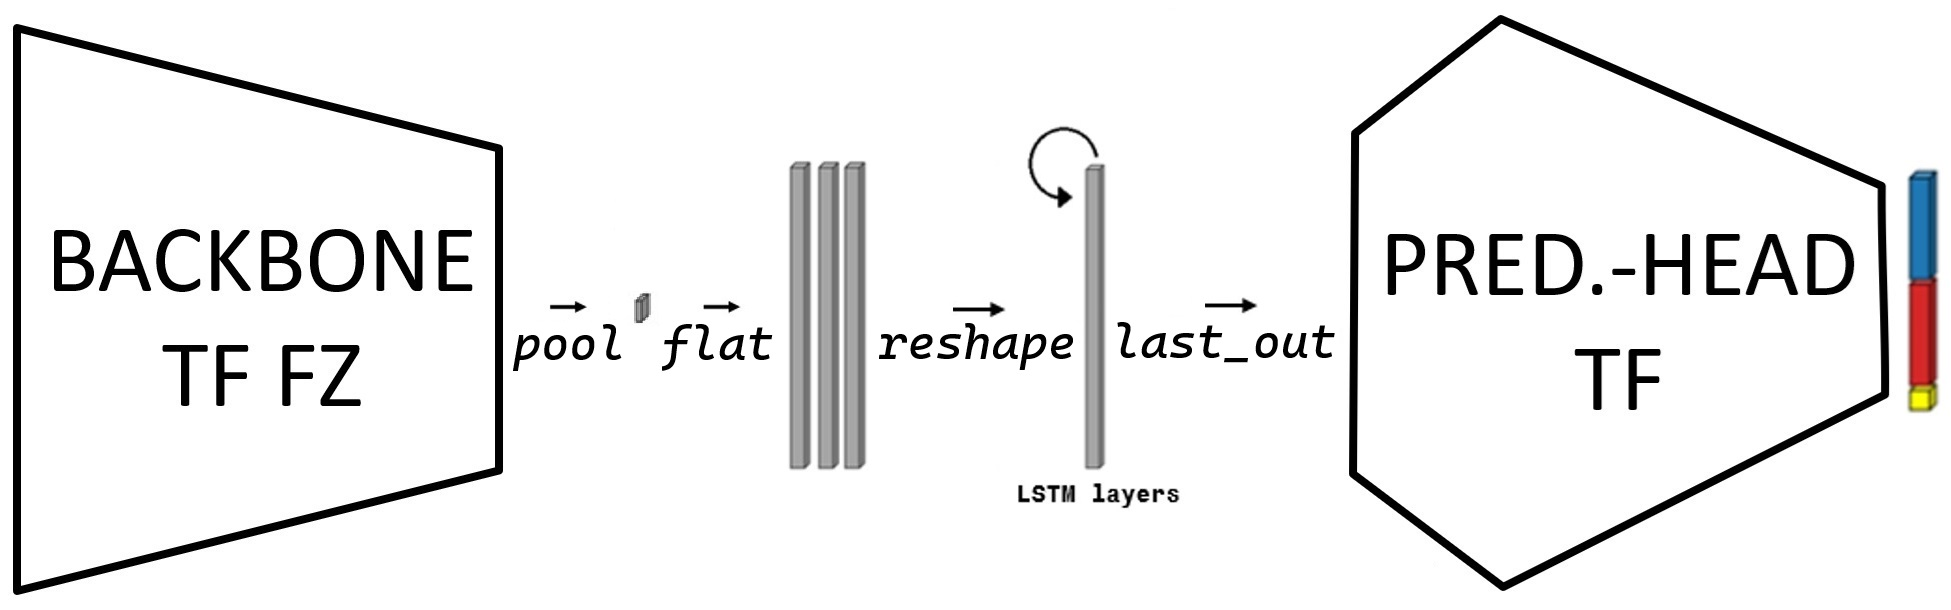
\includegraphics[width=\textwidth]{PICs/temporalModels/CNN_LSTM_FC.jpg}
        \caption{CNN\_LSTM\_FC}
    \end{subfigure}
    \hfill
    \begin{subfigure}[b]{0.48\textwidth}
        \centering
        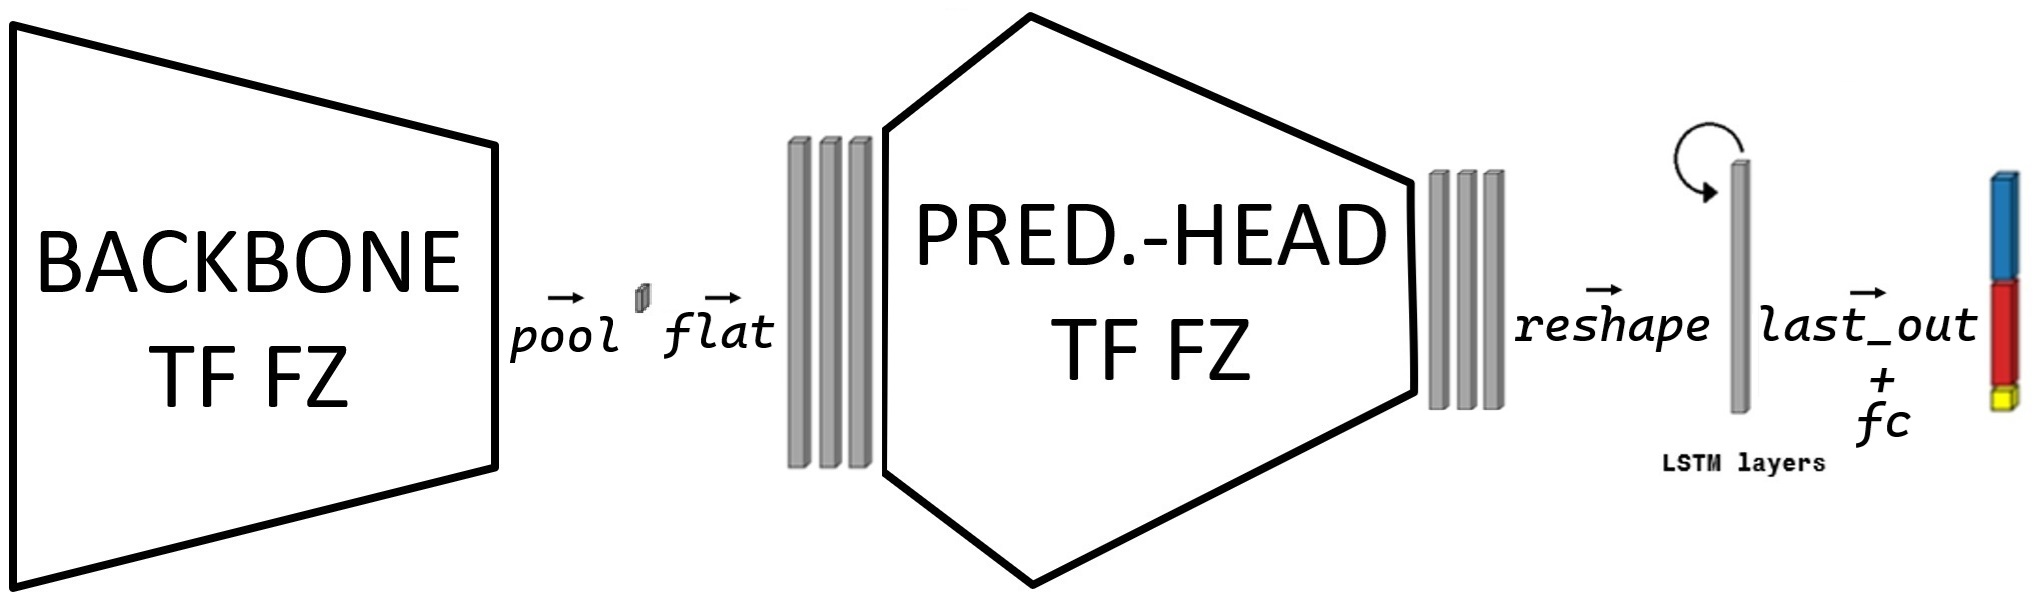
\includegraphics[width=\textwidth]{PICs/temporalModels/CNN_FC_LSTM.jpg}
        \caption{CNN\_FC\_LSTM}
    \end{subfigure}
    
    \vspace{0.5cm} % Abstand zwischen den Zeilen

    % Zweite Zeile
    \begin{subfigure}[b]{0.48\textwidth}
        \centering
        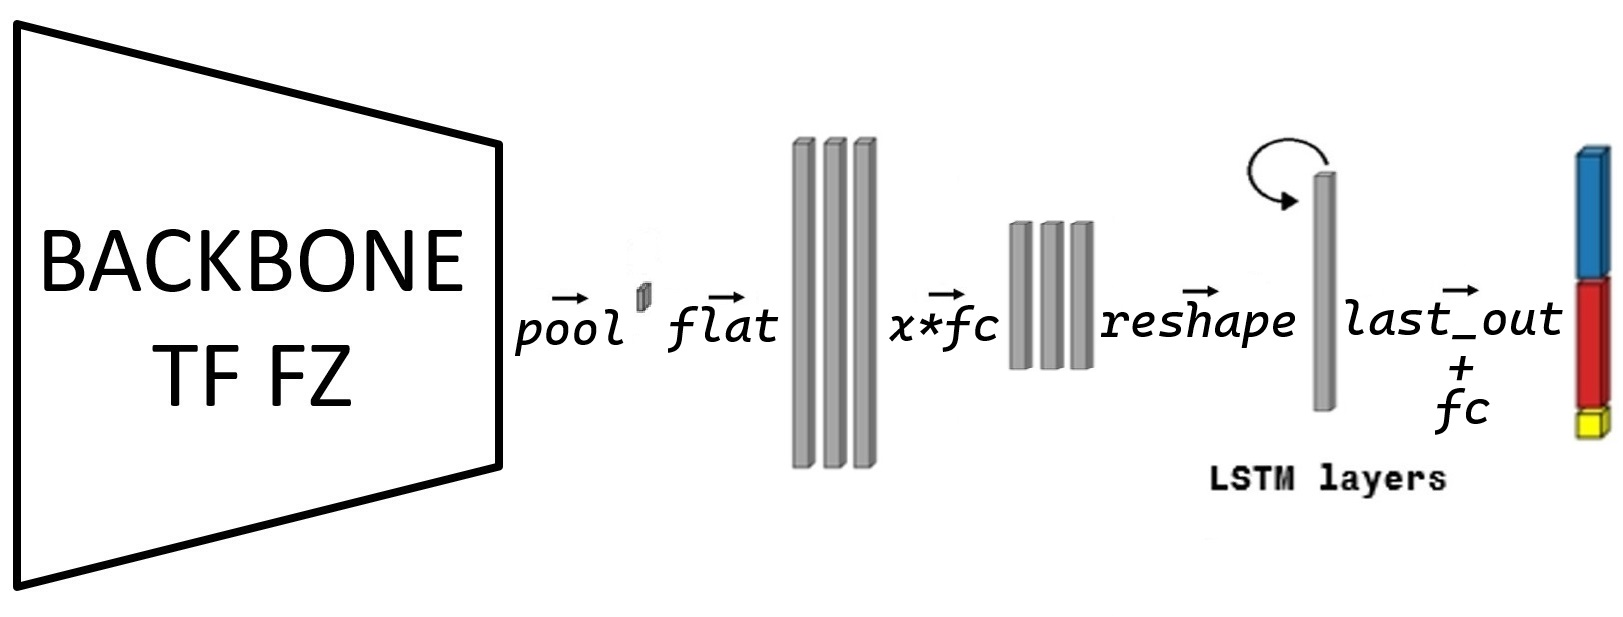
\includegraphics[width=\textwidth]{PICs/temporalModels/CNN_LSTM_V1_V2.jpg}
        \caption{CNN\_LSTM: $x=1$ (V1), $x=3$ (V2)}
    \end{subfigure}
    \hfill
    \begin{subfigure}[b]{0.48\textwidth}
        \centering
        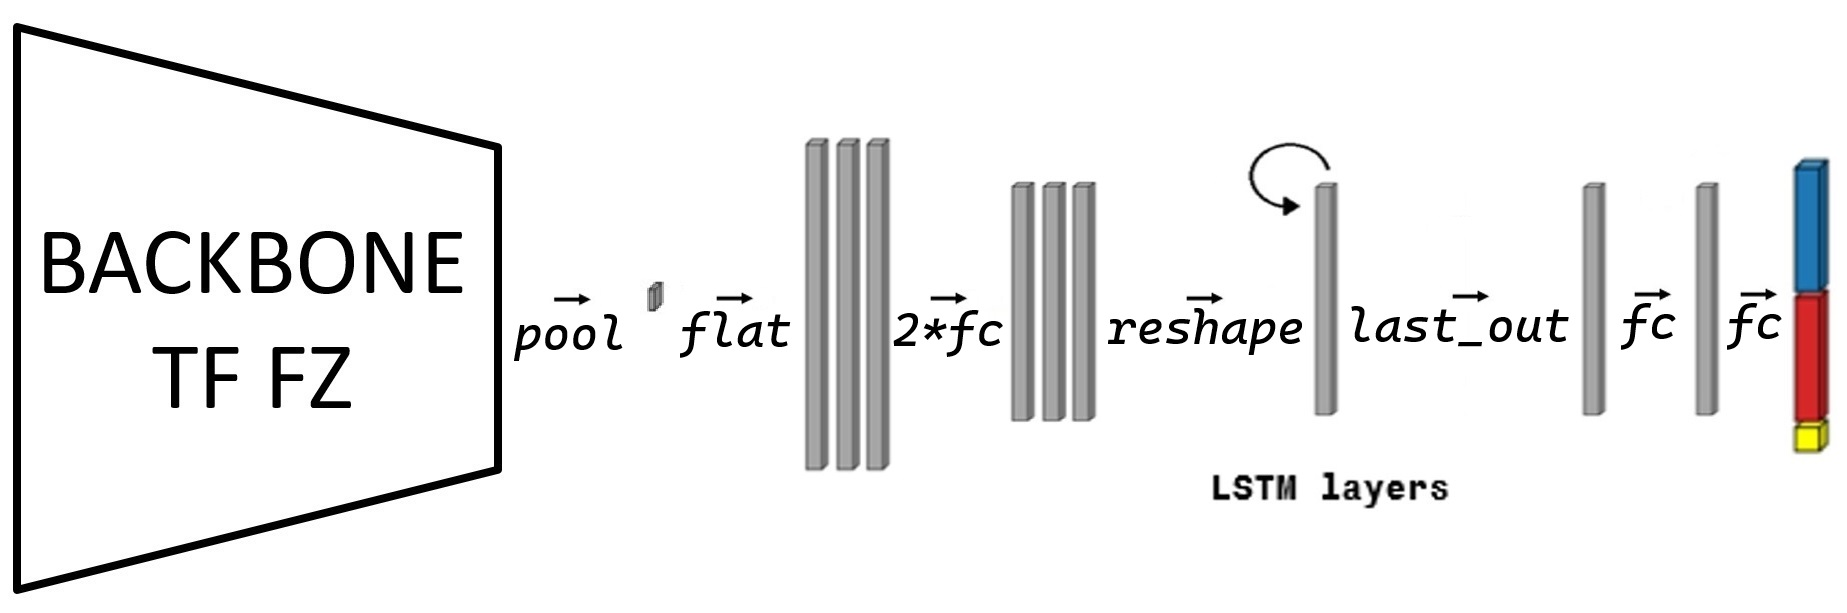
\includegraphics[width=\textwidth]{PICs/temporalModels/CNN_LSTM_HEAD.jpg}
        \caption{CNN\_LSTM\_HEAD}
    \end{subfigure}
    
    \vspace{0.5cm} % Abstand zwischen den Zeilen

    % Dritte Zeile
    \begin{subfigure}[b]{0.48\textwidth}
        \centering
        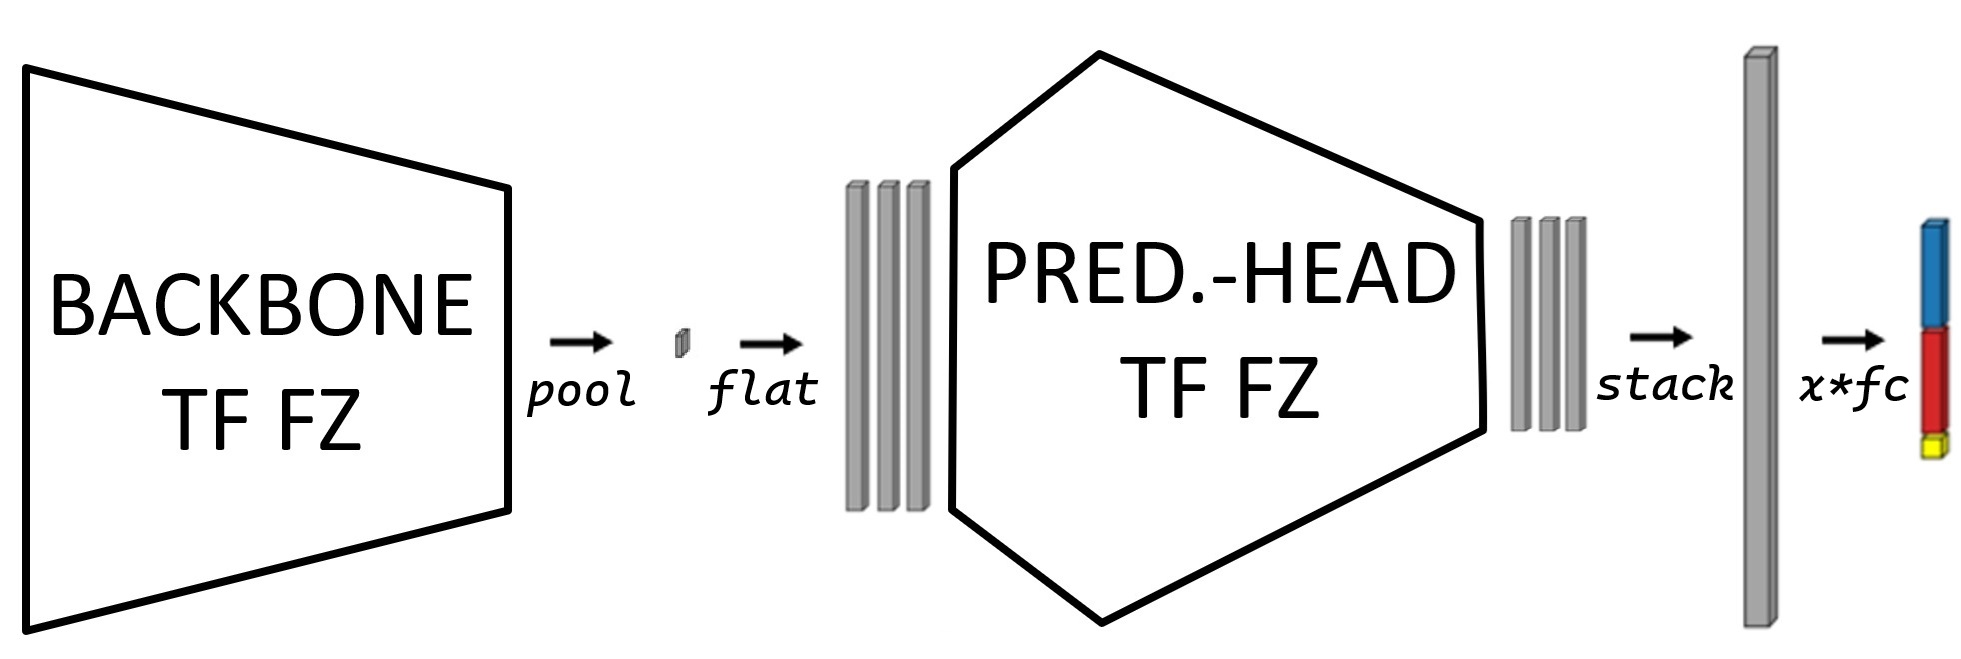
\includegraphics[width=\textwidth]{PICs/temporalModels/CNN_FC_FCOUT_V1_V2.jpg}
        \caption{CNN\_FC\_FCOUT: $x=1$ (V1), $x=3$ (V2)}
    \end{subfigure}
    \hfill
    \begin{subfigure}[b]{0.48\textwidth}
        \centering
        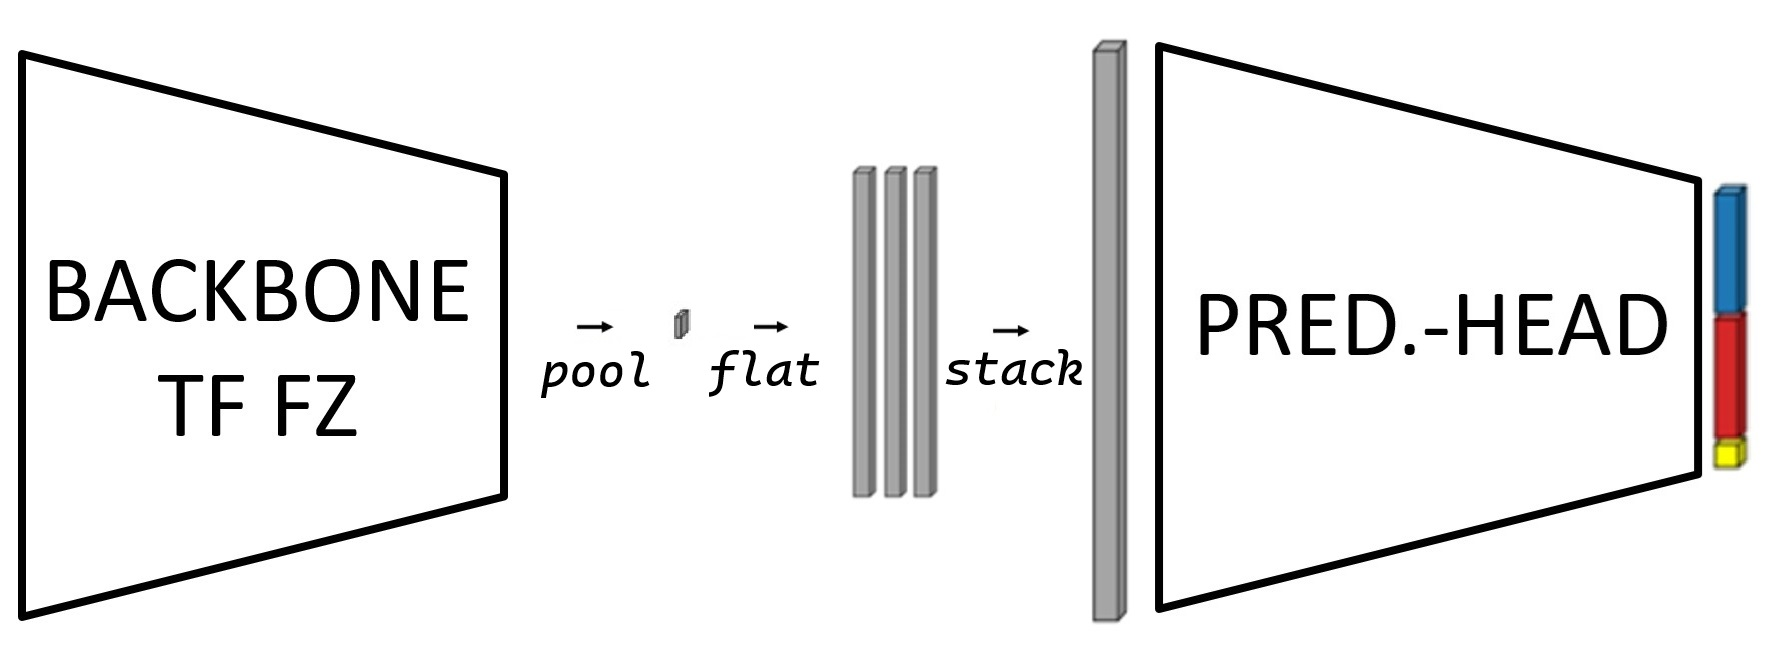
\includegraphics[width=\textwidth]{PICs/temporalModels/CNN_FLAT_FC.jpg}
        \caption{CNN\_FLAT\_FC}
    \end{subfigure}
    \caption{8 different temporal models for experiments. \textbf{(c)} and \textbf{(e)} have two versions in which the number of \ac{FC} layers vary. One \ac{FC} layer is used in for V1 and three Layers are used for the V2 model. Models \textbf{(a)}, \textbf{(b)}, \textbf{(c)} and \textbf{(d)} include LSTMs modules. Models \textbf{(e)} and \textbf{(f)} try to learn temporal dependencies only with \ac{FC} layers. Shape of heads resemble the architecture e.g. trapeze shaped contour is the trapeze head shown in \autoref{fig:predHeadTrapez}}
    \label{fig:temporalModels}
\end{figure}

Since the temporal modules need data in other formats, the logic of data processing before and within the model has to be changed as well.
The comparison between the data handling of single-frame training and the one proposed in this work for temporal training described in \autoref{sec:datahandling}.
In typical models that take single images into account, the network gets tensors with four dimensions consisting of batch size $B$, channels $C$, high $H$, and width $W$ also shown in \autoref{fig:backboneLogic}.
However, in this work, an additional dimension of the video stream length is introduced.
$S$ therefore defines how many sequential frames the model is fed with, resulting in a 5D tensor $[B, S, C, H, W]$.
Since the backbone is the same as the single-frame-based model it only supports 4D tensors shown in \autoref{fig:backboneLogic}.
For that reason, before the backbone, the tensor is transformed into a 4D one with the view function \cite{pytorch_view_docu}.
$B$ and $S$ are multiplied, resulting in $[B \times S, C, H, W]$.
This feature map is then processed by the backbone.
After flattening the tensor, only two dimensions remain $[B \times S, C]$.
In \autoref{fig:temporalModels} this feature map is visualized with three blocks indicating multiple feature maps from numerous images.
It stays that way until either a $reshape$ or a $stack$ transformation is conducted.
In this work, $reshaping$ is done by transforming $[B \times S, C]$ to $[B, S, C]$ as this form is needed for LSTMs.
$Stacking$, on the other hand, stacks the feature map into one big vector, resulting in a tensor where all images are in the $C$ dimension. 

LSTMs output sequence tensors with the same dimensions $[B, S, C]$.
Since only the features of the last sequence part are considered, the $last\_out$ transformation takes the channels of those images resulting in $[B, C]$ which is then further processed by \ac{FC} layers.
Even though almost all transformations support multi-batch training, to ease the logic all experiments with temporal models are done with a batch size of 1.
Similarly, when inferring these models a video stream consisting of multiple frames is transformed into a 4D tensor with dimensions $[S, C, H, W]$.
Therefore, to support inference this tensor must be extended with a batch size of 1 resulting in a tensor with dimensions $[1, S, C, H, W]$, which the model can take as input.
